% Fundamentação Teórica (Background) - CAP de extensão universitaria, CAP de curricularização da extensão, soluções/ferramentas de apoio a extensão (spoiler) se basear nas leis federais, resoluç~oes da unipampa (se aprofundar na previa do antreprojeto) como que a extensão funciona no Brasil, como é implantada nas universidades, o que foi a lei de curricularização, capitulo para falar da unipampa cidadã (Geral sobre extensão, tipos, perfis de pessoas, sempre com funcamentação. Programas e projetos de extensão na Unipampa (para demonstrar como é importante dentro da faculdade, impacto da ferramenta, graficos, valores)

%==============================================================================
\chapter{BACKGROUND}\label{background}
%==============================================================================
% 1 ou 2 paragrafos 

% ============================================================================
% Neste capitulo são discutidos assuntos assuntos que complementam o objetivo do presente trabalho, ajudando no entendimento das politicas e resoluções envolvidas. 
% Na \Cref{sec:3.1} sera apresentada a politica nacional de extensão, que vale para todo o Brasil sobre os objetivos que a extensão universitária tem em relação a comunidade academica e externa. 
% Logo em seguida na \Cref{sec:3.2} a visão de como a Unipampa se adaptou para receber estas novas regras. 
% Após, na \Cref{sec:3.2.1} a diferenca entre programas e projetos de extensão sera apresentada, seguido por uma explicação mais detalhada sobre o projeto 'Unipampa Cidadã' na \Cref{sec:3.2.2}. 
% A \Cref{sec:3.3} releva algumas ferramentas relacionadas ao assunto do trabalho, seus pontos em comum e uma descrição em alto nível. 
% Por fim na \Cref{sec:3.4} um resumo geral sobre o capitulo é apresentado.

This chapter discusses subjects that complement the objective of this work, helping to understand the policies and resolutions involved.
In \Cref{sec:3.1} the national outreach activity policy will be presented, which is valid for all of Brazil on the objectives that university outreach has in relation to the academic and external community.
Then in \Cref{sec:3.2} the vision of how Unipampa has adapted to receive these new rules.
After that, in \Cref{sec:3.2.1} the difference between outreach programs and projects will be presented, along with the most pertinent processes related to them in \Cref{sec:processes}, followed by a more detailed explanation about the ``Unipampa Cidadã'' project in \Cref{sec:3.2.3}.
The \Cref{sec:3.3} highlights some tools related to the subject of the work, their commonalities and a high-level description.
Finally in \Cref{sec:3.4} a general summary of the chapter is presented.
% ============================================================================

\section{National Outreach Policy}\label{sec:3.1}
% Descrever a politica em si
% ============================================================================
% Sabemos que a extensão universitária é uma area de grande importancia para a comunidade academica e externa, também sendo uma ferramenta de conexão entre professores, alunos e população, tendo muito impacto na formação de um estudante. 
% Para fortalecer os objetivos que a extensão universitaria tem dentro deste universo, o Fórum de Pró-Reitores de Extensão das Universidades Públicas Brasileiras (FORPROEX), acrescentou a versão antiga do documento da Politica Nacional de Extensão, publicado em 1999, com situações atuais e desafios encontrados nos ultimos anos. 
% A nova versão do documento, \cite{politicaNacional}, dentro dos seus objetivos, temos como exemplo os que seguem:

It is well-known that university outreach is an area of great importance for the academic and external community, also being a tool for connecting professors, students and the community, having a high impact on the soft skills a student formation. 
To strengthen the objectives that university outreach has within this universe, the \acl{FORPROEX} (\ac{FORPROEX}), updated the old version of the National Outreach Policy document, published in 1999, with current situations and challenges found in recent years.
The new version of the document, \cite{politicaNacional}, within its objectives, has as an example the following:
% ============================================================================

% ============================================================================
% \begin{itemize}
%     \item Conquistar o reconhecimento da extensão universitária, como uma ferramenta essencial para a universidade pública.
%     \item Garantir que a extensão seja a solução para qualquer tipo de problema social enfrentado pelo país.
%     \item Defender o financiamento de programas e projetos de extensão para que estes mantenham o seu funcionamento.
%     \item Promover a conscientização ambiental e sustentavel em projetos extensionistas no Brazil.
%     \item Além de nacionalmente, promover a solidariedade internacionalmente, abrangindo a aréa de impacto das ações extensionistas.
% \end{itemize}

\begin{itemize}
    \item Achieve the recognition of university outreach activities as an essential tool for the public university;
    \item Ensure that the outreach activity is the solution to any type of social problem faced by the country;
    \item Defend the funding of outreach programs and projects so that they can continue to function;
    \item Promote environmental and sustainable awareness in outreach projects in Brazil;
    \item Promote solidarity both nationally and internationally, covering the area of impact of outreach actions.
\end{itemize}
% ============================================================================

% ============================================================================
% Servindo como base para as universidades, o documento ``Referenciais para a construção de uma Política Nacional de Extensão nas ICES'' \cite{referenciaisPolitica}, 
% discute um pouco sobre a duvida da classificação de uma atividade academica como extensionista ou não, mas deixando como fato a seguinte frase ``Se a dimensão teórica da Extensão tende à maior rigidez - no sentido que precisa guardar princípios, retomar referenciais, 
% dialogar com outros documentos institucionais – a dimensão prática possibilita maior flexibilidade, originando uma considerável diversidade de ações''. 
% Este documento também destaca a importancia da integração da extensão com a pesquisa e ensino, com discussões de cunho social e efeitos dos resultados na sociedade.

Serving as a basis for universities, the document ``Referential for the construction of a National Outreach Policy in \aclp{HECI} (\ac{HECI})'' \cite{referenciaisPolitica},
discusses a little about the doubt of classifying an academic activity as outreach or not, but leaving as a fact the following sentence ``If the theoretical dimension of university outreach tends towards greater rigidity - in the sense that it needs to keep principles, resume references,
dialogue with other institutional documents – the practical dimension allows for greater flexibility, giving rise to a considerable diversity of actions'' \cite[p.43]{referenciaisPolitica}.
This document also highlights the importance of integrating outreach with research and teaching, with discussions of a social nature and the effects of the results on society.
% ============================================================================

% ============================================================================
% No documento supracitado, conjuntamente são aprofundados nove tipos de ações de extensão possíveis, cada um com suas peculiaridades, dividindo-as  em ações diretas de extensão e ações que permitem a integração entre extensão e ensino e extensão e pesquisa. 

As policy aforementioned, nine possible outreach activity types are discussed in depth, each with its peculiarities, dividing them into direct outreach actions and actions that allow the integration between outreach and teaching or outreach and research.

% ============================================================================

%https://sites.unipampa.edu.br/proext/documentos/politica-nacional-de-extensao/
% Plano Nacional de Educação 2014-2024 (Lei 13.005/2014)
% https://curricularizacaodaextensao.ifsc.edu.br/files/2016/06/1_Artigo_Curricularizaca_da_Extensao_Universitaria_no_Brasil.pdf
% FOREXT. Extensão nas Instituições Comunitárias de Ensino Superior: referenciais para a construção de
% uma Política Nacional de Extensão nas ICES (2013). Recuperado em 12 de março, 2015, em
% <http://www1.pucminas.br/imagedb/documento/DOC_DSC_NOME_ARQUI20150309182334.pdf>
% FORPROEX. Política Nacional de Extensão Universitária (2012). Recuperado em 12 de outubro, 2014,
% de <http://www.renex.org.br/documentos/2012-07-13-Politica-Nacional-de-Extensao.pdf>

\subsection{\acl{OA} Curricularization in Higher Education}\label{sec:3.1.1}
% Descrever aqui a ideia geral de como implementar isso dentro dos cursos pelas diferentes IESs
% ============================================================================
% Entrando no âmbito do ensino superior foi criado a Resolução Nº 7, de 18 de Dezembro de 2018 \cite{ministerioSuperiorExtensao}, aonde ela instituí diretrizes, princípios, fundamentos e procedimentos para a extensão na educação superior brasileira.
% Desta maneira foi regulamentado que as atividades de extensão serão disponibilizadas na forma de componentes curriculares para os cursos.

Entering the scope of higher education, Resolution No. 7, of December 18, 2018 \cite{ministerioSuperiorExtensao} was created, where it established guidelines, principles, foundations and procedures for university outreach in Brazilian higher education.
In this way, it was regulated that the \acp{OA} will be made available in the form of curricular subjects for the courses.
% ============================================================================

% ============================================================================
% Neste documento também é determinado que as atividades de extensão devem compor no minimo 10\% (dez por cento) de toda a carga horária dos cursos de graduação, sendo elas caracterizadas como uma atividade intervencionista que envolva diretamente a comunidade externa e esteja relacionada com a formação estudantil.

In this document, it is also determined that \acp{OA} must make up at least 10\% (ten percent) of the entire workload of undergraduate courses, being characterized as an interventionist activity that directly involves the external community and is related to student training.
% ============================================================================

% ============================================================================
% Outro ponto importante levantado, tem relação com a autoavaliação das atividades de extensão, para ocorrer ao aperfeicoamento constante da mesma. Nesta avaliação deverá ser incluido a identificação da pertinência da utilização das atividades de extensão na
% creditação curricular, a contribuição para o cumprimento dos objetivos do Plano de Desenvolvimento Institucional e dos Projetos Pedagógico dos Cursos e por fim a apresentação dos resultados conquistados em relação ao público participante.

Another important point raised is related to the self-assessment of outreach activities, in order to constantly improve it. 
This evaluation should include the identification of the relevance of the use of \acp{OA} in curricular accreditation, the contribution to the fulfillment of the objectives of the \ac{IDP} and the Pedagogical Projects of the Courses and, finally, the presentation of the results achieved in relation to the participating public.
% ============================================================================

% ============================================================================
% Todas as atividades de extensão também deverão ser registradas conforme as regras citadas na mesma resolução \cite{ministerioSuperiorExtensao}, devendo conter o planejamento de suas atividades internas, as estratégias para a autoavaliação, proposta, desenvolvimento e conclusão, estes devem estar devidamente registrados e analisados para poder ser feito a organização de seus planos de trabalho. 

All \acp{OA} must also be registered according to the rules mentioned in the same resolution \cite{ministerioSuperiorExtensao}, and must contain the planning of their internal activities, strategies for self-assessment, proposal, development and conclusion, these must be duly registered and analyzed in order to be able to organize your work plans.
% ============================================================================

% ============================================================================
% Por fim, a resolução supramencionada determina que ``As instituições de ensino superior terão o prazo de até 3 (três) anos, a contar da data de sua homologação, para a implantação do disposto nestas Diretrizes.''

Finally, the aforementioned resolution determines that ``Higher education institutions will have a period of up to 3 (three) years, counting from the date of their approval, to implement the provisions of these Guidelines.''
% ============================================================================

\section{\acl{OA} Curricularization in \acl{UNIPAMPA}} \label{sec:3.2}
% Descrever a visão da unipampa 
% https://sites.unipampa.edu.br/proext/documentos/normas-de-extensao-da-unipampa/
% https://sites.unipampa.edu.br/proext/files/2021/05/res-317_2021-politica-de-extensao.pdf
% - RESOLUÇÃO CONSUNI/UNIPAMPA Nº 317, DE 29 DE ABRIL DE 2021
% https://sites.unipampa.edu.br/proext/files/2021/12/sei_unipampa-0700488-resolucao-consuni.pdf
% - RESOLUÇÃO CONSUNI/UNIPAMPA Nº 332, DE 21 DE DEZEMBRO DE 2021

% Citar os cases de sucesso como ES e outros cursos de Uruguaiana

% ============================================================================
% Estando na visão da Unipampa, ela como todas as universidades federais, deve ter uma resolução voltada para a normatização para as atividades de extensão de modo geral apresentando o que elas são, seu publico alvo, objetivos etc. 
% Tendo em vista isso a Unipampa na Resolução CONSUNI/UNIPAMPA Nº 332 de 2021, \cite{Resolucao-332:2021}, determina os tipos de atividades de extensão, ja mencionados na \Cref{introduction}, seus orgãos gerenciadores, equipe executora, possíveis processos relacionados, e algumas regras como a de duração mínima de 8 (oito) horas, levando-se em conta o período de organização, execução e elaboração de relatório final.

In \ac{UNIPAMPA}'s view, like all other \acl{HEI}, must have a resolution aimed at standardizing \acp{OA} in general, presenting what they are, their target audience, objectives, etc.
In view of this, \ac{UNIPAMPA}, in CONSUNI/UNIPAMPA Resolution No. 332 of 2021, \cite{Resolucao-332:2021}, determines the types of outreach activities, already mentioned in \Cref{introduction}, its managing bodies, executing team, possible related processes, and some rules such as the minimum duration of 8 (eight) hours, taking into account the period of organization, execution and preparation of the final report.
% ============================================================================

% ============================================================================
% A algum tempo a Unipampa ja vem implantando alguns projetos de extensão dentro de sua grade curricular, por exemplo no curso de Engenharia de Software onde dentro da cadeira de Resolução de Problemas, os alunos se reunem em grupos, semelhante a times de desenvolvimento e gerencia de projetos, sendo eles designados para trabalhar em uma demanda real para alguém da comunidade externa. 
% Esta atividade proporciona ao aluno uma experiência muito recompensadora, pela oportunidade de falar, interagir e contribuir diretamente com um cliente que necessita de ajuda na resolução de algum problema.

For some time now, \ac{UNIPAMPA} has been implementing some outreach projects within its curriculum, for example in the Software Engineering course where, within the Problem Solving subject, students meet in groups, similar to development teams and project management, where they are assigned to work on real demand for someone in the external community.
This activity provides the student with a very rewarding experience, for the opportunity to talk, interact and contribute directly with a customer who needs help in solving a problem.

% ============================================================================

% ============================================================================
% Os principais objetivos na inserção das atividades extensionistas nos cursos de graduação, que a Unipampa ressalta em sua Resolução Nº 317 de 2021, \cite{res317} são os seguintes: 
% \begin{itemize}
%   \item Ajudar ao discente desenvolver sua formação crítica, cidadã, interdisciplinar e responsável;
%   \item Aprimorar como um todo o ensino nos cursos de graduação e fortalecer aa indissociabilidade entre ensino, pesquisa e extensão;
%   \item Fortalecer o compromisso social da Unipampa; 
%   \item Estimular discussões construtivas em todos os setores da Unipampa; 
%   \item Promover ações que fortifiquem os princípios éticos, e o compromisso social da Unipampa em todas as áreas;
%   \item Instigar a comunidade academica a estar mais presente no desenvolvimento humano, academico, social, cultural e economico.
% \end{itemize}

The main objectives in the insertion of outreach activities in undergraduate courses, which \ac{UNIPAMPA} highlights in its Resolution No. 317 of 2021, \cite{res317} are the following:
\begin{itemize}
  \item Help students develop their critical, citizen, interdisciplinary and responsible education;
  \item Improve teaching in undergraduate courses as a whole and strengthen the inseparability among teaching, research and outreach;
  \item Strengthen \ac{UNIPAMPA}'s social commitment;
  \item Stimulate constructive discussions in all sectors of \ac{UNIPAMPA}; 
  \item Promote actions that strengthen \ac{UNIPAMPA}'s ethical principles and social commitment in all areas;
  \item Encourage the academic community to be more present in human, academic, social, cultural, and economic development.
\end{itemize}
% ============================================================================

\subsection{Outreach Programs and Projects}\label{sec:3.2.1}
% Diferença entre eles
% Citar exemplos de Prog. e Proja. dos cursos do campus

% ============================================================================
% Para explicar o que são programas e projetos de extensão, sera utilizado as definições da \textcite{referenciaisPolitica}, este diz que são atividades reguladas internamente pela instituição que articula eventos envolvendo ensino e pesquisa, sempre envolvendo a comunidade externa. 
% Com eles os alunos podem tomar atitudes e decisões diretamente sobre a comunidade em que vive, contribuindo na evolução e progresso da mesma. 
% Além de ajudar a comunidade externa, \ac{FOREXT} diz que os programas e projetos não buscam criar um laço de dependência com a universidade, sendo assim é necessário resolver o problema com mais eficácia e qualidade possível.

To explain what outreach projects and programs are, the definitions of \textcite{referenciaisPolitica} will be used, which says that they are activities regulated internally by the institution that articulates events involving teaching and research, always involving the external community.
With them, students can take attitudes and decisions directly about the community in which they live, contributing to its evolution and progress.
In addition to helping the external community, \ac{FOREXT} says that the programs and projects do not seek to create a bond of dependence with the university, so it is necessary to solve the problem with the most efficiency and quality possible.

% ============================================================================

% ============================================================================
% Pelo fato dos dois termos serem semelhantes, alguma confusão pode acontecer, então \textcite{Viero} destaca a diferença entre os dois, citando as definições feitas pela \ac{ProExt}:

Because the two terms are similar, some confusion can arise, so \textcite{Viero} highlights the difference between the two, citing the definitions made by \ac{ProExt}:
% ============================================================================

% ============================================================================
% \begin{citacao}
% É importante salientar que o ProExt prevê dois conjuntos de ações de extensão universitária: projetos de extensão, definidos como “conjunto de ações processuais contínuas, de caráter educativo, social, cultural ou tecnológico, com objetivo específico e prazo determinado”; e programa de extensão, como “conjunto articulado de projetos e outras ações de extensão, preferencialmente de caráter multidisciplinar e integrado a atividades de pesquisa e de ensino \cite{Viero}
% \end{citacao}

\begin{citacao}
It is important to point out that ProExt provides for two sets of university outreach actions: outreach projects, defined as “a set of continuous procedural actions, of an educational, social, cultural or technological nature, with a specific objective and a determined period”; and outreach program, as “an articulated set of projects and other outreach actions, preferably of a multidisciplinary nature and integrated with research and teaching activities \cite{Viero}.
\end{citacao}
% ============================================================================

% ============================================================================
% Dentro da \ac{UNIPAMPA} campus Alegrete existem alguns projetos e programas vigentes, são exemplos deles com os seus respectivos coordenadores: 
% \begin{inparaenum}[(1)]
%   \item \textbf{Ciência a Cavalo: Universidade e Ensino Básico de Mãos Dadas pelo Fortalecimento da Educação}, Marco Antonio Durlo Tier;
%   \item \textbf{Consultoria de TI para empresas do agronegócio}, Elder de Macedo Rodrigues;
%   \item \textbf{Empresa Júnior: Multi Assessoria e Soluções em Engenharia Júnior - Masé Junior}, José Gabriel Vieira Neto;
%   \item \textbf{Espaço Maker} - Aprendizagem criativa, Vitor Almada;
%   \item \textbf{Programa UniHacker.Club}, Diego Luiz Kreutz;
%   \item \textbf{UNIPATAS Alegrete: Proteção, Esterilização e Adoção}, Camila da Costa Lacerda Tolio Richardt;
%   \item \textbf{Programa C}, Aline Vieira de Mello;
%   \item \textbf{Programa JEDI}, Maicon Bernardino da Silveira.
% \end{inparaenum}

% ########################
% Professor, fiquei em dúvida se traduzia os nomes dos programas de extensão, dai eu traduzi so o que eu achei que não fazia parte do nome em si.
% ########################
Within the \ac{UNIPAMPA} Alegrete campus there are some current projects and programs, examples of which are with their respective coordinators:
\begin{inparaenum}[(1)]
  \item \textbf{Ciência a Cavalo: University and Basic Education Hand in Hand for Strengthening Education}, Profº Marco Antonio Durlo Tier;
  \item \textbf{IT consultancy for Agribusiness Companies}, Profº Elder de Macedo Rodrigues;
  \item \textbf{Empresa Júnior: Multi Advisory and Solutions in Junior Engineering - MASE Junior}, Profº José Gabriel Vieira Neto;
  \item \textbf{Espaço Maker} - Criative Learning, TAE Vitor Almada;
  \item \textbf{Programa UniHacker.Club}, Profº Diego Luiz Kreutz;
  \item \textbf{UNIPATAS Alegrete: Protection, Sterilization and Adoption}, TAE Camila da Costa Lacerda Tolio Richardt;
  \item \textbf{Programa C}, Profª Aline Vieira de Mello;
  \item \textbf{Programa JEDI}, Profº Maicon Bernardino da Silveira.
\end{inparaenum}
% ============================================================================

% ============================================================================
% Utilizando a página online do ultimo programa citado \textcite{JEDI}, este é um programa que se propoe a resolver problemas locais utilizando tecnologia e envolvimento com a comunidade. 
% No primeiro ciclo do programa quatro projetos de extensão foram propostos, cada um com seus objetivos, metodologias e atividades próprios, são eles:
% \begin{inparaenum}[(1)]
%   \item Padawan Academy;
%   \item Jedi Apprentice;
%   \item Jedi Problem-Solving;
%   \item Jedi Mind.
% \end{inparaenum}

% Using the online page of the last mentioned program \textcite{JEDI}, this is a program that proposes to solve local problems using technology and community involvement.
% In the first cycle of the program, four outreach projects were proposed, each with its own objectives, methodologies and activities, they are:
% \begin{inparaenum}[(1)]
%   \item Padawan Academy;
%   \item Jedi Apprentice;
%   \item Jedi Problem-Solving;
%   \item Jedi Mind.
% \end{inparaenum}

% ============================================================================

\subsection{Processes for New Proposals for Outreach Programs and Projects}\label{sec:processes}

% ============================================================================
% Para ser realizado o novo cadastro de um programa ou projeto de extensão e sua geração de certificados ao final, existem algumas normas definidas pela \textcite{Resolucao-332:2021}, que devem ser desempenhados antes. 
% Tendo em maos estes documentos a \ac{UNIPAMPA} normatizou alguns esquemas de fluxo dos processos, para que todos os proponentes tenham conhecimento do que acontece depois que a proposta é realizada.

In order to register a new outreach program or project and generate certificates at the end, there are some rules defined by \textcite{Resolucao-332:2021}, which must be performed beforehand.
With these documents in hand, \ac{UNIPAMPA} standardized some process flow schemes, so that all proponents are aware of what happens after the proposal is made.
% ============================================================================

% ============================================================================
% Na \Cref{fig:outreach-projects-registration}, o fluxo de cadastro de um novo projeto de extensão é apresentado, nele é possivel ver que a proposta passa por diversos passos de correções e avaliações, sendo enviada para diversos atores ao longo do processo.
% Por fim sendo decisão da \ac{PROEXT} solicitar alterações finais, ou homologar o projeto, deferindo um novo número de registro.

In \Cref{fig:outreach-projects-registration}, the registration flow of a new outreach project is presented, in which it is possible to see that the proposal goes through several steps of corrections and evaluations, being sent to several actors throughout the process.
% ============================================================================

\begin{figure}[htb]
  \caption{Outreach Projects Registration}\label{fig:outreach-projects-registration}
  \begin{center}
    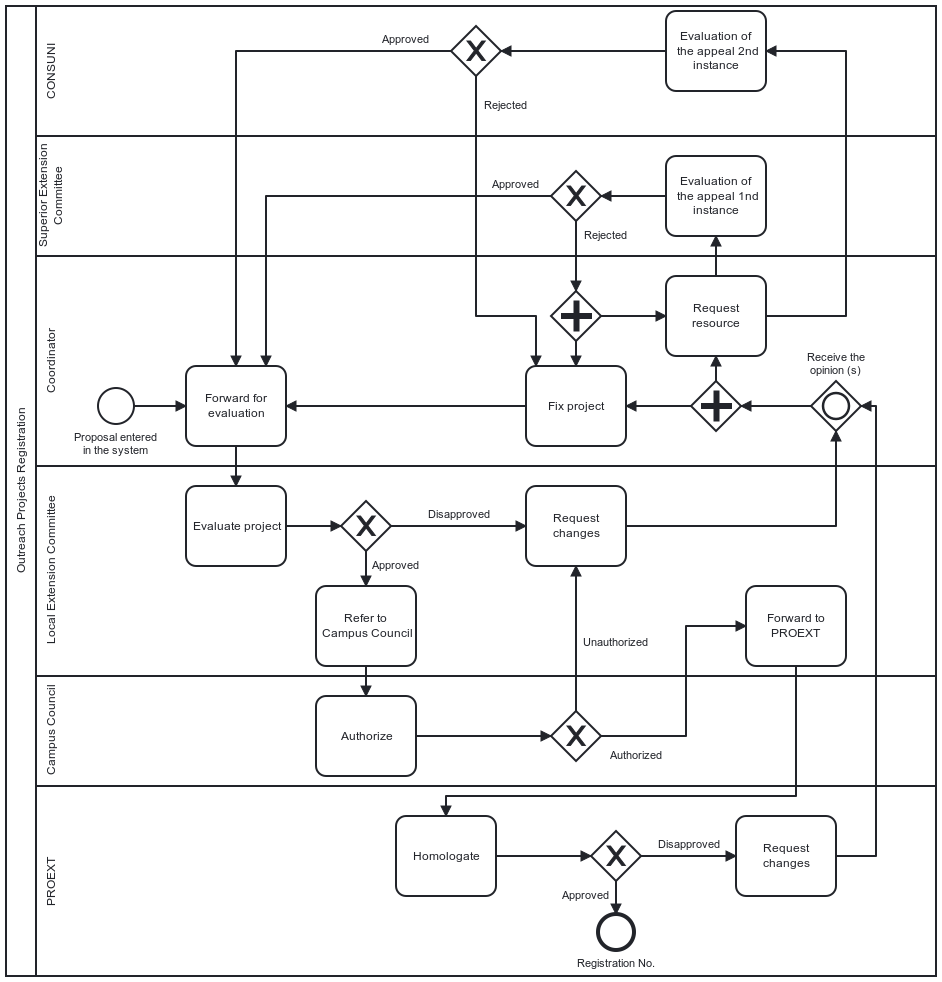
\includegraphics[width=16cm]{img/3-registro-de-projetos-de-extensao.png}
  \end{center}
  \fonte{Adapted from \cite{siteProcessos}.}
\end{figure}

% ============================================================================
% Já na \Cref{fig:issuance-certificates}, estão representados os passos relacionados a homologação e geração de certificados, comecando com o proponente da atividade tendo em maõs a lista de presença e a planilha com informações para a geração dos certificados, logo um relatorio final é construido e inserido no sistema \ac{SIPPEE}, este é avaliado e homologado, chegando novamente até a \ac{PROEXT} que com a planilha enviada, envia seus dados para o sistema \ac{SGCE}, recebendo os certificados e os enviando para os emails dos participantes. 

In \Cref{fig:issuance-certificates}, the steps related to the approval and generation of certificates are represented, starting with the proponent of the activity having the attendance list and the spreadsheet with information for the generation of certificates. 
Then, a final report is built and inserted in the \ac{SIPPEE} system, it is evaluated and approved, reaching again at \ac{PROEXT} which, with the spreadsheet sent, sends its data to the \ac{SGCE} system, receiving the certificates and sending them to participants' emails.
% ============================================================================

\begin{figure}[htb]
  \caption{Issuance of certificates}\label{fig:issuance-certificates}
  \begin{center}
    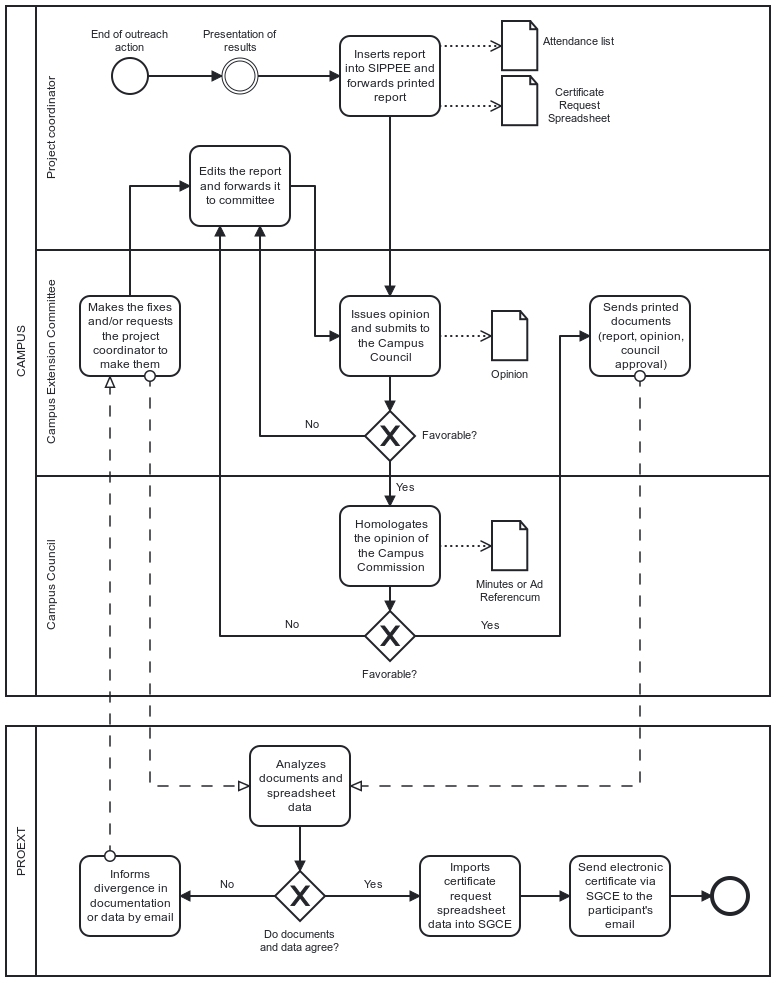
\includegraphics[width=16cm]{img/3-emissao-de-certificados.png}
  \end{center}
  \fonte{Adapted from \cite{siteProcessos}.}
\end{figure}

\subsection{``Unipampa Cidadã'' Program}\label{sec:3.2.3}
% https://unipampa.edu.br/portal/sites/default/files/documentos/instrucao_normativa_18-2021_revoga_in-17-2021_normatiza_o_programa_institucional_unipampa_cidada.pdf
% INSTRUÇÃO NORMATIVA UNIPAMPA Nº 18, 05 DE AGOSTO DE 2021

% ============================================================================
% A \ac{UNIPAMPA} atravez da Instrução Normativa Nº 18 \cite{unipampacidada}, usando a Resolução Nº317 \cite{res317}, foi estabelecido que o projeto de extensão chamado "UNIPAMPA Cidadã" deverá ser ofertado por todos os cursos, sendo composto por atividades de cidadania e solidariedade e com o objetivo de  formar egressos cientes de sua responsabilidade social, estimulando e aumentando a integração com a comunidade local.

\ac{UNIPAMPA} through Normative Instruction No. 18 \cite{unipampacidada}, using Resolution No.317 \cite{res317}, established that the outreach project called ``Unipampa Cidadã'' must be offered by all courses, consisting of citizenship and solidarity activities and with the objective of training graduates aware of their social responsibility, stimulating and increasing integration with the local community.
% ============================================================================

% ============================================================================
% Após a implementação do projeto nos cursos da instituição, esta deverá ser realizada por todos os discentes, a cadeira ofertada para o projeto deverá ter no mínimo 60 e no máximo 120 horas. 
% As ações comunitárias devem ser realizadas em instituições públicas, \acp{NGO} e organizações ou associações da sociedade civil organizada. O supervisor de extensão do curso é o encarregado por fazer a avaliação do projeto, planejamento, acompanhamento, validação e ele será responável por aprovar o inicio das atividades.

After the implementation of the project in the institution's courses, it must be carried out by all students, the course offered for the project must have a minimum of 60 and a maximum of 120 hours.
Community actions must be carried out in public institutions, \acp{NGO} and organizations or associations of organized civil society. 
The course outreach supervisor is responsible for carrying out the project evaluation, planning, monitoring, validation and he will be responsible for approving the beginning of the activities.
% ============================================================================

% ============================================================================
% O projeto também disponibiliza na Instrução Normativa Nº 18, um modelo de formulário para preenchimento de dados quando as atividades são finalizadas, permitindo o discente refletir sobre o impacto do projeto sob sua visão apontando seus aprendizados durante a execução. 
% Por fim o supervisor pode realizar observaçoes sobre o discente e indicar se este foi aprovado ou reprovado.

The project also makes available in Normative Instruction Nº 18, a form template for filling in data when the activities are completed, allowing the student to reflect on the impact of the project under their view, pointing out what they learned during the execution.
Finally, the supervisor can make observations about the student and indicate whether he or she passed or failed.
% ============================================================================
\section{Similar Outreach Support Tools}\label{sec:3.3}
% Overview de soluções
% Descrever em alto nível e fazer gancho (spoiler) com o Capítulo do grey
% Funcionalidades comuns
% Foi feito um detalhamento metodologico no capitulo 4.1
% Tentamos fazer revisão sistematica, encontramos duas mas preferimos a cinza
% Citar artigos que falam do ferramental

% ============================================================================
% Em conjunto com o \Cref{cap:grey} que ira apresentar a revisão conduzida na literatura cinza, algumas ferramentas foram pesquisadas para adiquirir informaçoes de como o mercado está em relaçao a extensão nas universidades. 
% Com os resultados foi possível levantar funcionalidades, detalhes e pontos em comum dentre as ferramentas.

In conjunction with \Cref{grey_literature} that will present the review conducted in the grey literature, some tools were researched to acquire information on how the market is in relation to outreach in universities.
With the results it was possible to raise functionalities, details and common points among the tools.
% ============================================================================

% ============================================================================
% Em um primeiro momento os autores buscaram fazer uma revisão sistematica na literatura branca, mas os resultados encontrados não satisfazeriam por completo, visto que a exploração manual por várias ferramentas relacionadas ao tema, traria mais conteúdo para ser classificado e discutido entre os envolvidos na pesquisa.

At first, the authors sought to make a systematic review of the white literature, but the results found would not be completely satisfactory, since the manual exploration by various tools related to the topic would bring more content to be classified and discussed among those involved in the research.
% ============================================================================

% ============================================================================
% Durante a execução da revisão, a ferramenta que mais retornou resultados e estava sempre presente nas pesquisas, foi a \ac{SIGAA}, a qual é a mais utilizada por diversas instituições, sendo ela muito completa contendo partes em seu sistema voltados para a maioria dos processos que envolvem uma instituição. 
% Outra que apresentou resultados interessantes foi a \ac{CAEX}, que apresentou diversas funcionalidades únicas, sendo apenas ela que as apresentava, com ela foi possível retirar ideias de grande importancia para a construção de uma ferramenta completa.

During the execution of the review, the tool that returned the most results and was always present in the research was \ac{SIGAA}, which is the most used by several institutions, being very complete, containing parts in its system aimed at most processes involving an institution.
Another one that presented interesting results was \ac{CAEX}, which presented several unique features, being only it that presented them, with this it was possible to extract ideas of great importance for the construction of a complete tool.
% ============================================================================
\section{Chapter Summary}\label{sec:3.4}
% ============================================================================
% Neste capítulo foi apresentado diretrizes de varias resoluçoes e normativas relacionadas a extensão, tanto no pais como um todo, quanto na \ac{UNIPAMPA}. 
% Também foi discutido sobre as semelhanças e diferenças entre os termos programa e projeto de extensão, apresentando os processos mais relevantes envolvidos no seu periodo de vida.
% Como exemplo mais recente de programa de extensão, a "UNIPAMPA Cidadã" teve parte de seus objetivos e diretrizes apresentados, por fim foi discutido um pouco sobre a revisão na literatura cinza executada pelos participantes desta pesquisa, logo no proximo capítulo será mais aprofundado critérios, metodologia, resultados, questões de pesquisa, dentre outras informaçoes pertinentes a literatura cinza.

In this chapter, guidelines of various resolutions and regulations related to outreach were presented, both in the country as a whole and in \ac{UNIPAMPA}.
It was also discussed the similarities and differences between the terms outreach program and project, presenting the most relevant processes involved in its life span.
As a more recent example of an outreach program, ``Unipampa Cidadã'' had part of its objectives and guidelines presented, finally, a little discussion about the grey literature review carried out by the participants of this research was discussed, so in the next chapter, criteria will be more in-depth, methodology, results, research questions, among other information relevant to grey literature.
% ============================================================================